\documentclass{article}

\usepackage[UTF8, scheme = plain]{ctex}
\usepackage{fancyhdr}
\usepackage{extramarks}
\usepackage{amsmath}
\usepackage{amsthm}
\usepackage{amsfonts}
\usepackage{tikz}
\usepackage[plain]{algorithm}
\usepackage{algpseudocode}
\usepackage{color}
\usepackage{listings}
\usepackage{fontspec}
\usepackage{float}

\newfontfamily\menlo{Menlo}
% \newfontfamily\menlo{Consolas}
\lstset{
    columns=fixed,       
    numbers=left,                                        % 在左侧显示行号
    numberstyle=\tiny\color{gray},                       % 设定行号格式
    frame=none,                                          % 不显示背景边框
    backgroundcolor=\color[RGB]{245,245,244},            % 设定背景颜色
    keywordstyle=\color[RGB]{40,40,255},                 % 设定关键字颜色
    numberstyle=\footnotesize\color{darkgray},           
    commentstyle=\it\color[RGB]{0,96,96},                % 设置代码注释的格式
    stringstyle=\rmfamily\slshape\color[RGB]{128,0,0},   % 设置字符串格式
    showstringspaces=true,                              % 不显示字符串中的空格
    numberstyle=\small\menlo,
    basicstyle=\small\menlo,
    breaklines=true,
}

% \lstset{
%     language=Octave,                % the language of the code
%     basicstyle=\footnotesize,           % the size of the fonts that are used for the code
%     numbers=left,                   % where to put the line-numbers
%     numberstyle=\tiny\color{gray},  % the style that is used for the line-numbers
%     stepnumber=1,                   % the step between two line-numbers. If it's 1, each line 
%                                     % will be numbered
%     numbersep=5pt,                  % how far the line-numbers are from the code
%     backgroundcolor=\color{white},      % choose the background color. You must add \usepackage{color}
%     showspaces=false,               % show spaces adding particular underscores
%     showstringspaces=false,         % underline spaces within strings
%     showtabs=false,                 % show tabs within strings adding particular underscores
%     frame=single,                   % adds a frame around the code
%     rulecolor=\color{black},        % if not set, the frame-color may be changed on line-breaks within not-black text (e.g. commens (green here))
%     tabsize=2,                      % sets default tabsize to 2 spaces
%     captionpos=b,                   % sets the caption-position to bottom
%     breaklines=true,                % sets automatic line breaking
%     breakatwhitespace=false,        % sets if automatic breaks should only happen at whitespace
%     title=\lstname,                 % show the filename of files included with \lstinputlisting;
%                                     % also try caption instead of title
%     keywordstyle=\color{blue},          % keyword style
%     commentstyle=\color{dkgreen},       % comment style
%     stringstyle=\color{mauve},         % string literal style
%     escapeinside={\%*}{*)},            % if you want to add LaTeX within your code
%     morekeywords={*,...}               % if you want to add more keywords to the set
% }

\usetikzlibrary{automata,positioning}

%
% Basic Document Settings
%
%%% page layout
\topmargin=-0.45in
\evensidemargin=0in
\oddsidemargin=0in
\textwidth=6.5in
\textheight=9.0in
\headsep=0.25in

\linespread{1.1}    %%% line spacing

\definecolor{ustcblue}{cmyk}{1,0.8,0,0}

\pagestyle{fancy}
\lhead{\hmwkAuthorName}
\chead{\hmwkClass\ (\hmwkClassInstructor): \hmwkTitle}
\rhead{}
\lfoot{}
\cfoot{\thepage}

\renewcommand\headrulewidth{0.4pt}
\renewcommand\footrulewidth{0.4pt}

\setlength\parindent{0pt}

%
% Create Problem Sections
%

\newcommand{\enterProblemHeader}[1]{
    \nobreak\extramarks{}{Problem \arabic{#1} continued on next page\ldots}\nobreak{}
    \nobreak\extramarks{Problem \arabic{#1} (continued)}{Problem \arabic{#1} continued on next page\ldots}\nobreak{}
}

\newcommand{\exitProblemHeader}[1]{
    \nobreak\extramarks{Problem \arabic{#1} (continued)}{Problem \arabic{#1} continued on next page\ldots}\nobreak{}
    \stepcounter{#1}
    \nobreak\extramarks{Problem \arabic{#1}}{}\nobreak{}
}

\setcounter{secnumdepth}{0}
\newcounter{partCounter}
\newcounter{homeworkProblemCounter}
\setcounter{homeworkProblemCounter}{1}
\nobreak\extramarks{Problem \arabic{homeworkProblemCounter}}{}\nobreak{}

%
% Homework Problem Environment
%
% This environment takes an optional argument. When given, it will adjust the
% problem counter. This is useful for when the problems given for your
% assignment aren't sequential. See the last 3 problems of this template for an
% example.
%
\newenvironment{homeworkProblem}[1][-1]{
    \ifnum#1>0
        \setcounter{homeworkProblemCounter}{#1}
    \fi
    \subsection{Exercise \arabic{homeworkProblemCounter}}
    \setcounter{partCounter}{1}
    \enterProblemHeader{homeworkProblemCounter}
}{
    \exitProblemHeader{homeworkProblemCounter}
}

%
% Homework Details
%   - Title
%   - Due date
%   - Class
%   - Section/Time
%   - Instructor
%   - Author
%

\newcommand{\hmwkTitle}{Homework\ \#1}
\newcommand{\hmwkDueDate}{\today}
\newcommand{\hmwkClass}{Engineering Seismology}
\newcommand{\hmwkClassInstructor}{Professor B. Wang}
\newcommand{\hmwkAuthorName}{\textbf{Jintao Li}}
\newcommand{\hmwkAuthorID}{\textbf{SA20007037}}
\newcommand{\hmwkAuthoremail}{\textbf{E-mail: lijintao@mail.ustc.edu.cn}}

%
% Title Page
%

% \title{
%     \vspace{2in}
%     \textbf{\hmwkClass:\ \hmwkTitle}\\
%     \normalsize\vspace{0.2in}\large{\hmwkDueDate}\\
%     \vspace{0.2in}\large{\textit{\hmwkClassInstructor}}
%     \vspace{3in}
% }

% \author{\hmwkAuthorName \\
% \hmwkAuthorID}
% \date{}

\renewcommand{\part}[1]{\textbf{ \\ (\alph{partCounter})  }\stepcounter{partCounter} }

%
% Various Helper Commands
%

% Useful for algorithms
\newcommand{\alg}[1]{\textsc{\bfseries \footnotesize #1}}

% For derivatives
\newcommand{\deriv}[1]{\frac{\mathrm{d}}{\mathrm{d}x} (#1)}

% For partial derivatives
\newcommand{\pderiv}[2]{\frac{\partial}{\partial #1} (#2)}

% Integral dx
\newcommand{\dx}{\mathrm{d}x}

% Alias for the Solution section header
\newcommand{\solution}{\textbf{\large \\ Solution: \\}}

% Probability commands: Expectation, Variance, Covariance, Bias
\newcommand{\E}{\mathrm{E}}
\newcommand{\Var}{\mathrm{Var}}
\newcommand{\Cov}{\mathrm{Cov}}
\newcommand{\Bias}{\mathrm{Bias}}

%
\newcommand{\mb}[1]{\mathbf{#1}}

\begin{document}

\begin{titlepage}

\begin{center}

\textcolor{ustcblue}{
\includegraphics[width=0.4\textwidth]{./ustc_logo_fig.pdf} \\ [1cm]}
% Title
{ \Huge \bfseries \hmwkClass}\\[1cm]
{\Huge \bfseries \hmwkTitle} \\[1cm]

\large \textbf{\hmwkClassInstructor} \\ [5cm]

\large \hmwkAuthorName \\ [0.25cm]
\large \hmwkAuthorID \\ [0.25cm]
\large \hmwkAuthoremail
\vfill
% Bottom of the page
% {\large March 24, 2021}
{\large \today}

\end{center}

\end{titlepage}

\begin{center}
\section{第五讲:强震观测数据及处理}
\end{center}

\begin{homeworkProblem}[1]
搜集2019年7月Ridgecrest Mw7.1地震100km以内强震数据

\solution

数据下载:
\begin{itemize}
    \item [1. ]
    打开网址:{\color{blue}{https://www.strongmotioncenter.org/iqr1.php}},见下图
    \begin{figure}[H]
        \centering
        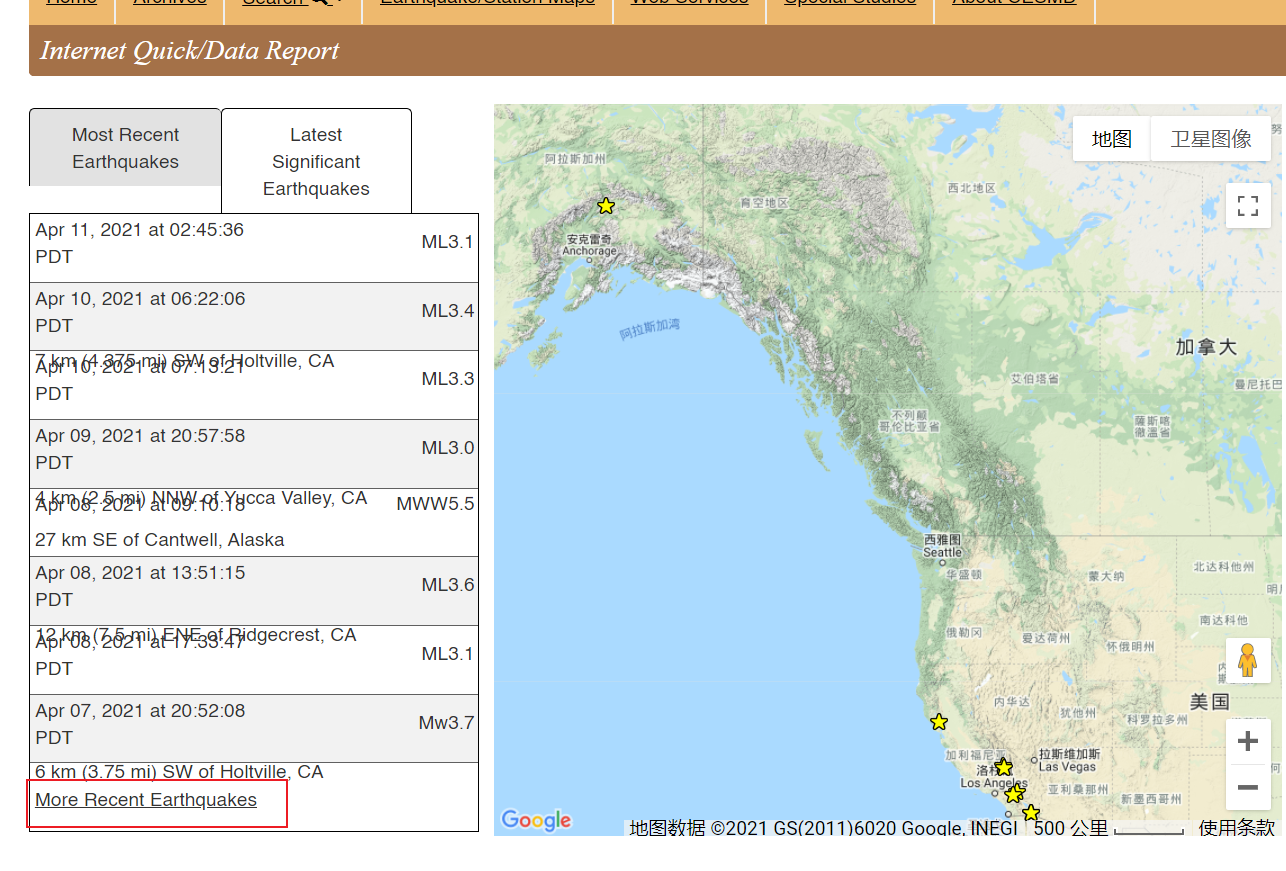
\includegraphics[width=4in, keepaspectratio]{figure/01.png}
        \label{fig:f01}
    \end{figure}
    \item [2. ]
    点击下方的 "More Recent Earthquakes",然后选择时间为 2019(见下图)。
    \begin{figure}[H]
        \centering
        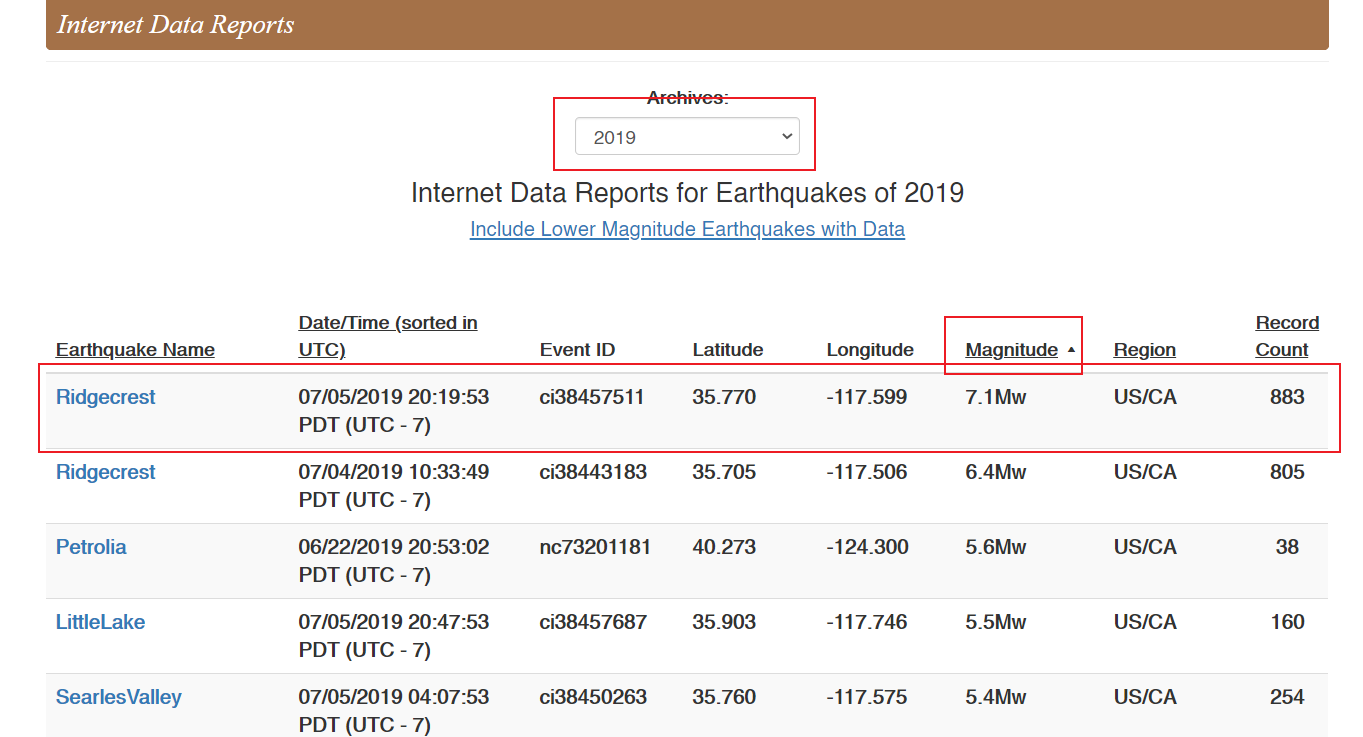
\includegraphics[width=4in, keepaspectratio]{figure/02.png}
        \label{fig:f02}
    \end{figure}
    \item [3. ]
    点击 "Magnitude",使地震按照震级大小排序,然后位列第一个的地震就
是2019年7月Ridgecrest Mw7.1地震(见上图描述)。
    \item [4. ]
    点击左侧的 "Ridgecrest" 进入台站页面,网页的上面会显示该地震的基本信息:震级、
时间、坐标等(见下图)。
然后点击 "Epic.",使台站按照震中距排序,一个发现31个100km
以内的台站,选择这些台站,然后点击 "Download" 下载(有些台站数据的通道不同,所以最终只选用了28个台站),
见下图。

\begin{figure}[H]
    \centering
    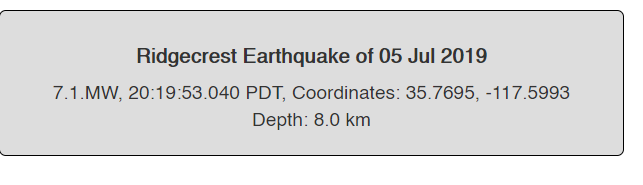
\includegraphics[width=4in, keepaspectratio]{figure/03.png}
    \label{fig:f03}
\end{figure}
\begin{figure}[H]
    \centering
    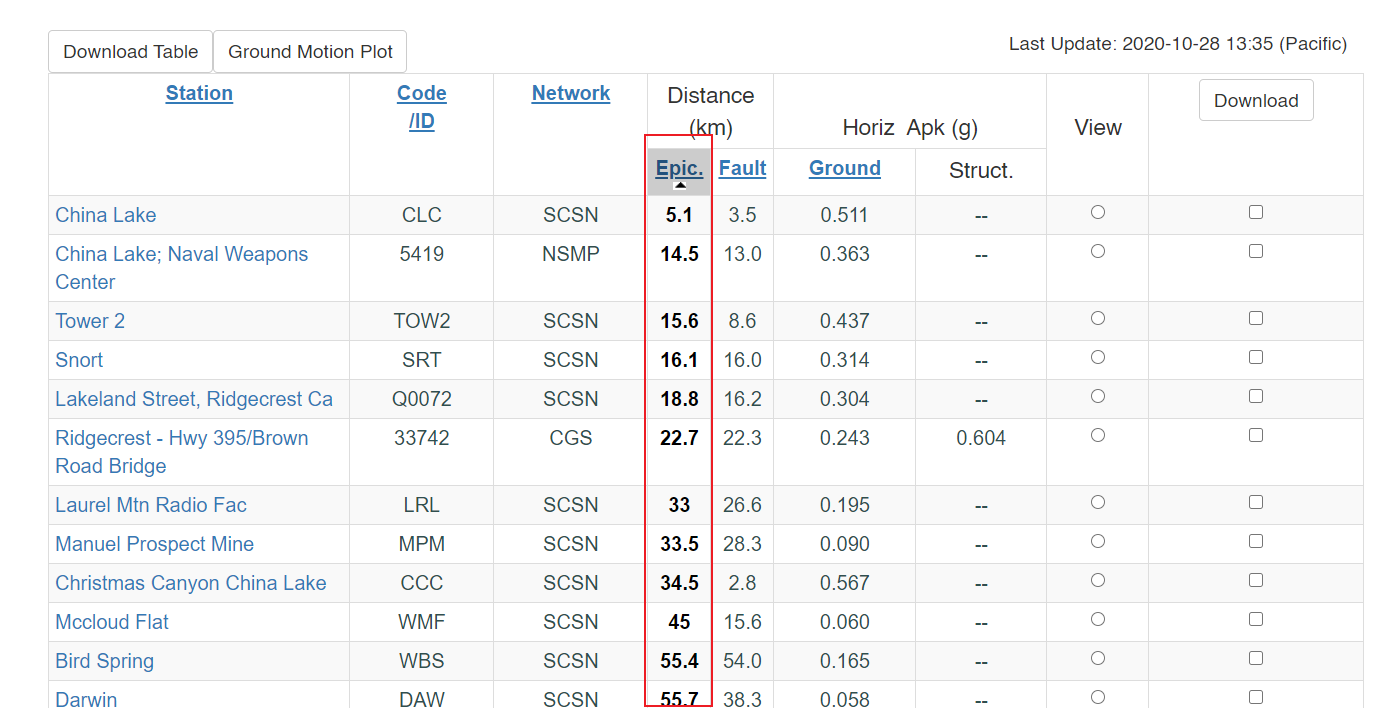
\includegraphics[width=4in, keepaspectratio]{figure/04.png}
    \label{fig:f04}
\end{figure}
\item [5. ]
    选择 "Processed Data" 下载(见下图)。Processed Data 是处理好的数据,
'.v2' 文件里面已经储存了加速度、速度、位移等信息。
\begin{figure}[H]
    \centering
    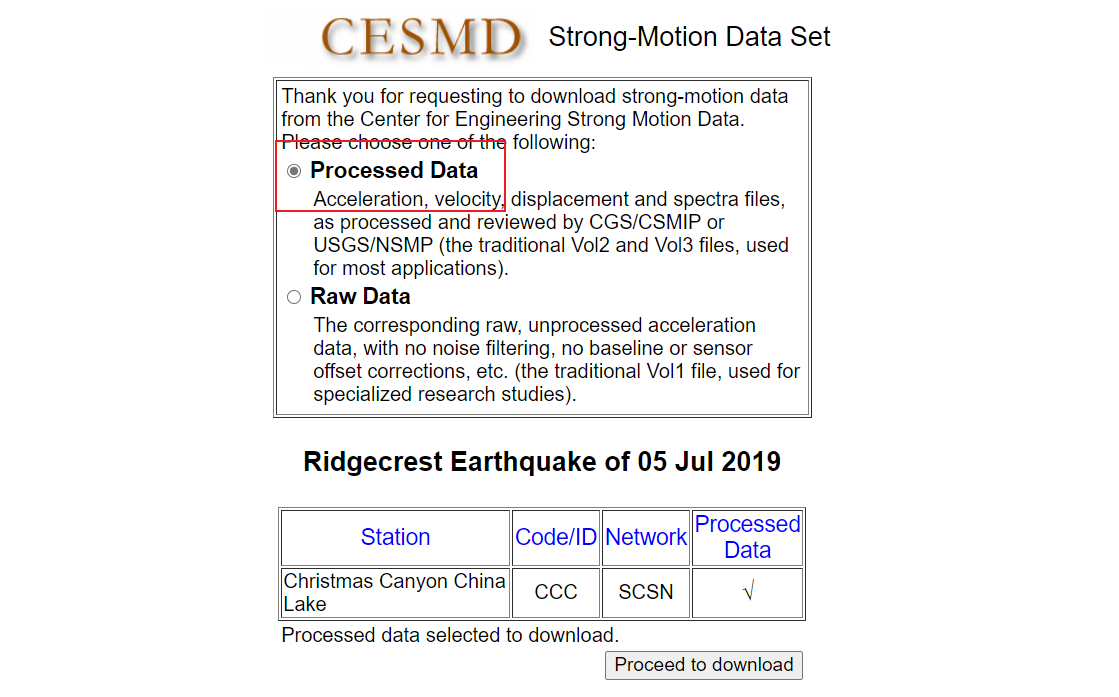
\includegraphics[width=4in, keepaspectratio]{figure/05.png}
    \label{fig:f05}
\end{figure}
\end{itemize}

\end{homeworkProblem}

\pagebreak


\begin{homeworkProblem}[2]
分析PGA,PGV,PGD以及持时随距离的分布

\solution

在 ".v2" 文件中已经包含了PGA、PGV、PGD的信息。每一个 ".v2" 文件,里面有三个通道,分别为 
"360"、"up"、"90" (由于有几个台站的通道不属于这三个,所以我们弃用那几个台站的信息),
而 PGA、PGV、PGD 就分别在自每一个通道起始位置开始(此处记为1)的
第18、19、20行,如下图所示。
\begin{figure}[H]
    \centering
    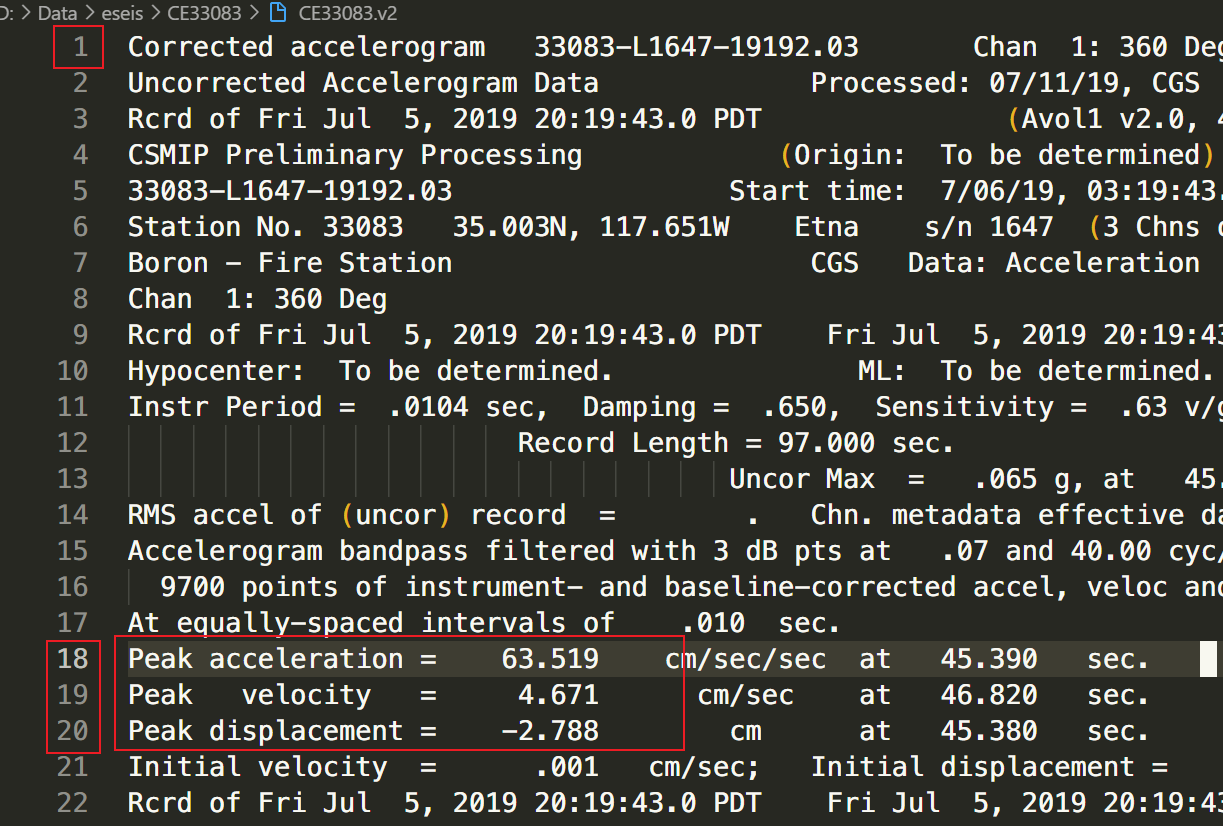
\includegraphics[width=3in, keepaspectratio]{figure/06.png}
    \label{fig:f06}
\end{figure}

每一个通道以 "/\&" 所在的一行结尾,我们可以用 python 脚本读取每一个文件的 PGA、PGV、
PGD(实际上,我们不仅读取了这三个数据,还把台站的经纬度读了出来,由于文件命名混乱,我们直接使用台站和
震中的经纬度计算震中距,没有使用网站上的距离,实际上在保留两位小数的情况下,两者误差不超过0.1km)。\\

\textbf{python code}
\begin{lstlisting}[language={python}]
def readpeak(filename):
    f = open(filename)
    lines = f.readlines()

    pga = []
    pgv = []
    pgd = []
    loc = [0]
    i = 0
    for line in lines:
        if line[:2] == '/&':
            loc.append(i+1)
        i = i+1

    assert (len(loc) == 4)

    for i in loc[:3]:
        pga.append(float(lines[i + 17].split()[3]))
        pgv.append(float(lines[i + 18].split()[3]))
        pgd.append(float(lines[i + 19].split()[3]))

    return pga, pgv, pgd
\end{lstlisting}

\pagebreak

一般来说,有三种方式计算持续时间,我们选用第三种,即 $90\%$ 能量持续的时间。
使用 python 脚本读取 v2 文件中的所有加速度,然后使用以下公式计算持续时间:
\begin{equation}
    I(t)=\int_{0}^{t} a^{2}(t) d t / \int_{0}^{T} a^{2}(t) d t
\end{equation}

最后我们可以得到结果:
\begin{figure}[H]
    \centering
    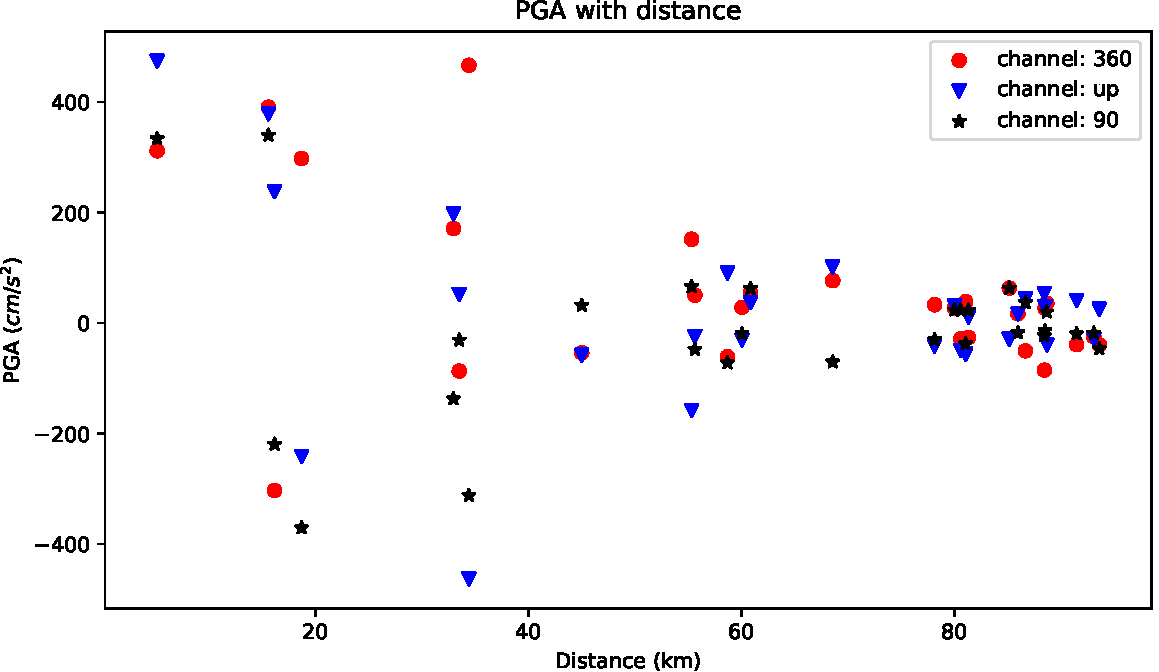
\includegraphics[width=4in, keepaspectratio]{figure/pga.pdf}
    \label{fig:pga}
\end{figure}
\begin{figure}[H]
    \centering
    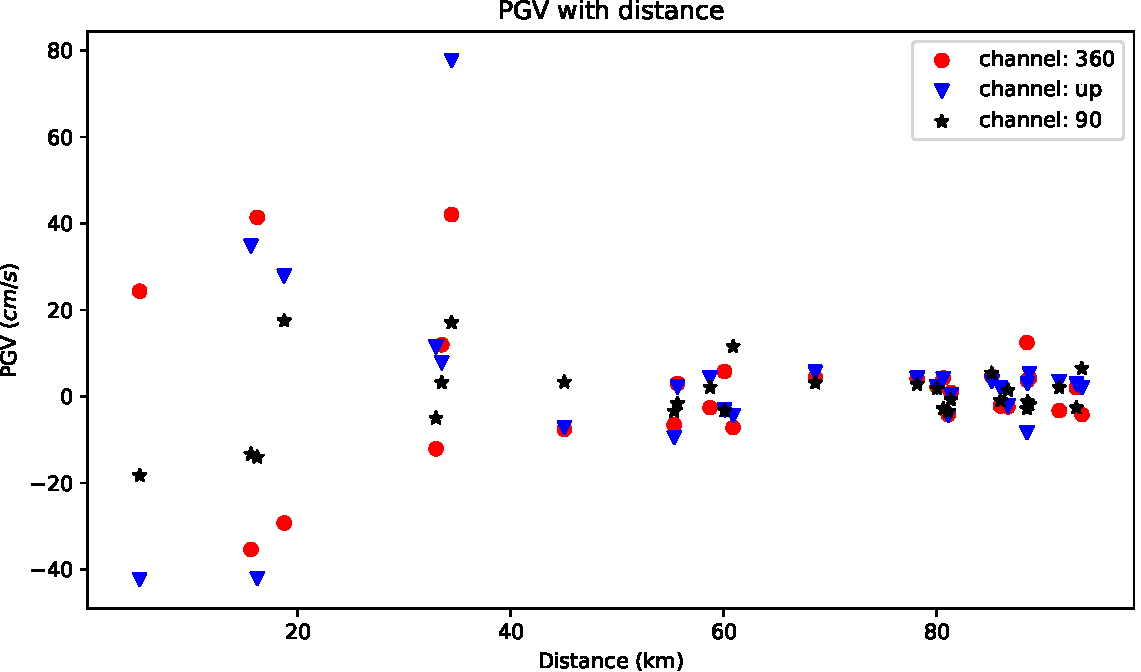
\includegraphics[width=4in, keepaspectratio]{figure/pgv.pdf}
    \label{fig:pgv}
\end{figure}
\begin{figure}[H]
    \centering
    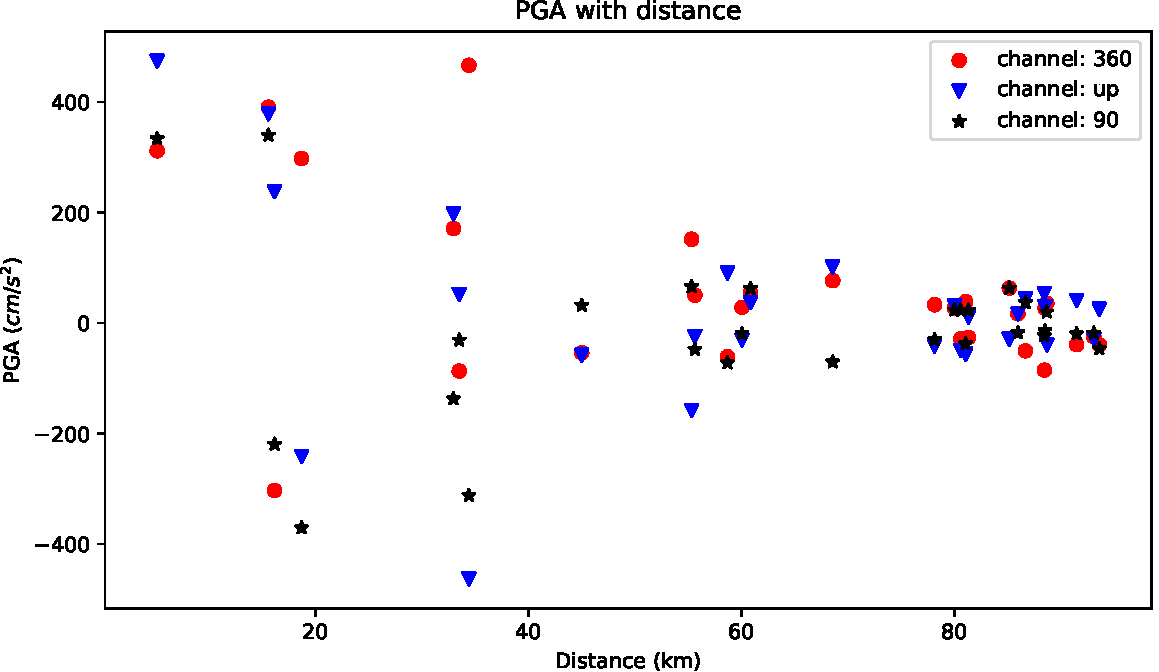
\includegraphics[width=4in, keepaspectratio]{figure/pga.pdf}
    \label{fig:pgd}
\end{figure}
\begin{figure}[H]
    \centering
    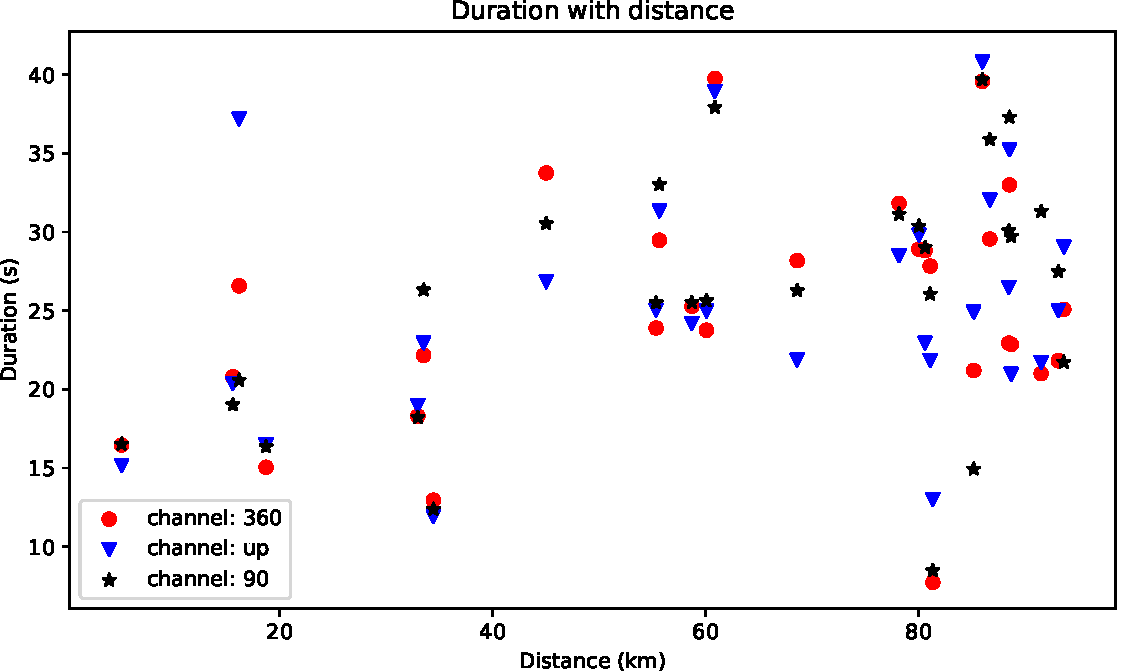
\includegraphics[width=4in, keepaspectratio]{figure/duration.pdf}
    \label{fig:duration}
\end{figure}

从上述四张图中,我们可以看出,PGA、PGV、PGD 的振幅大小(即绝对值)随着距离的增大逐渐减小,最后趋于0。
这是很好理解的,因为离震中越远,地震对该地的影响就越小,所以 PGA、PGV、PGD 的振幅大小会逐渐变小。
持续时间的趋势不太好区分,但大体上是随着距离增大而增大。


\end{homeworkProblem}

\pagebreak

\begin{homeworkProblem}[3]
根据最近的一个台站计算反应谱

\solution

最近的一个台站是距离震中 5.1 km 的 China Lake 台站,谱数据存储在 v3 文件。
使用 python 脚本读取 v3 文件数据,并绘图(去掉了谱数据末尾的几个0)。
得到的结果与使用 ViewWave 软件得到的结果相似度很高,结果可信。
实验结果如下图所示:

\begin{figure}[H]
    \centering
    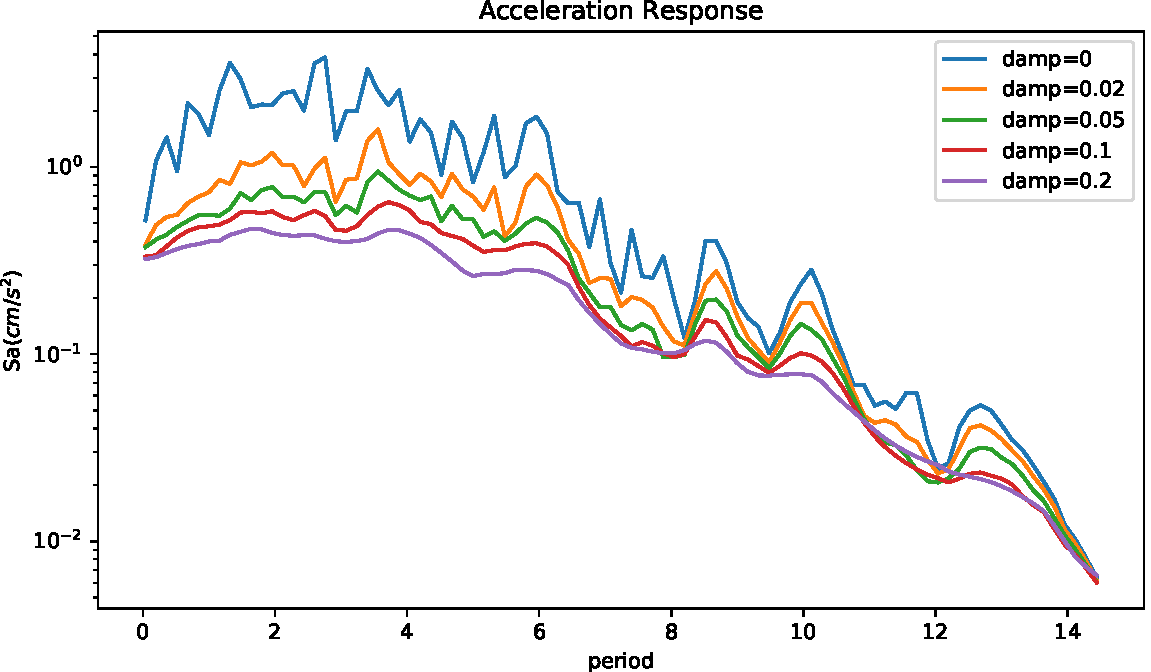
\includegraphics[width=4in, keepaspectratio]{figure/sa.pdf}
    \label{fig:sa}
\end{figure}
\begin{figure}[H]
    \centering
    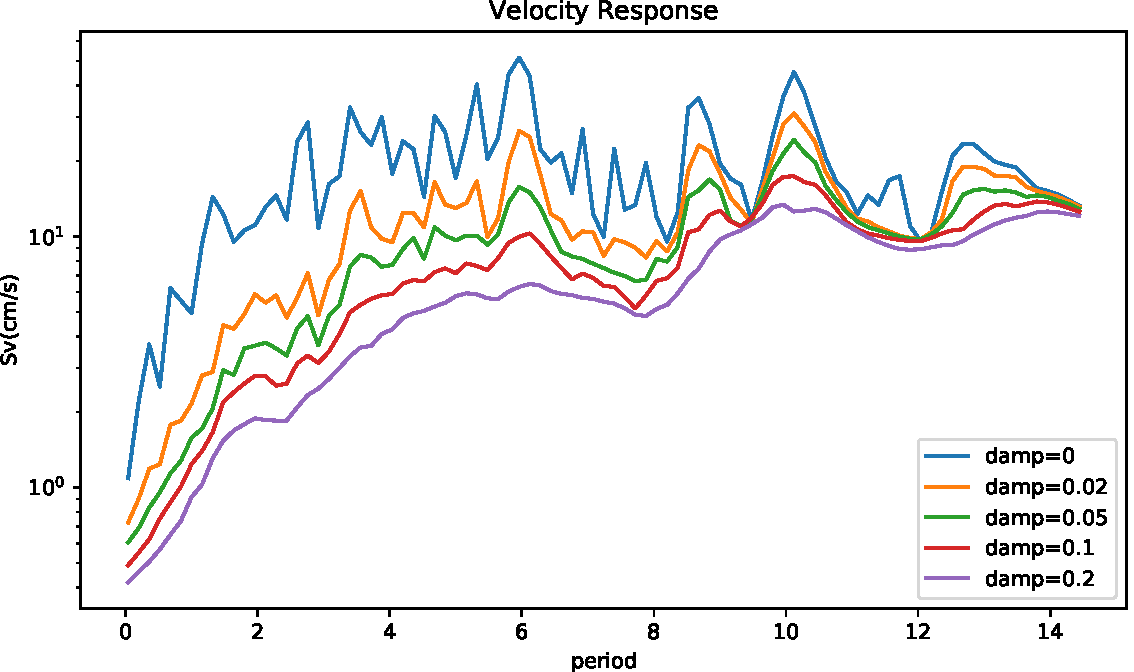
\includegraphics[width=4in, keepaspectratio]{figure/sv.pdf}
    \label{fig:sv}
\end{figure}
\begin{figure}[H]
    \centering
    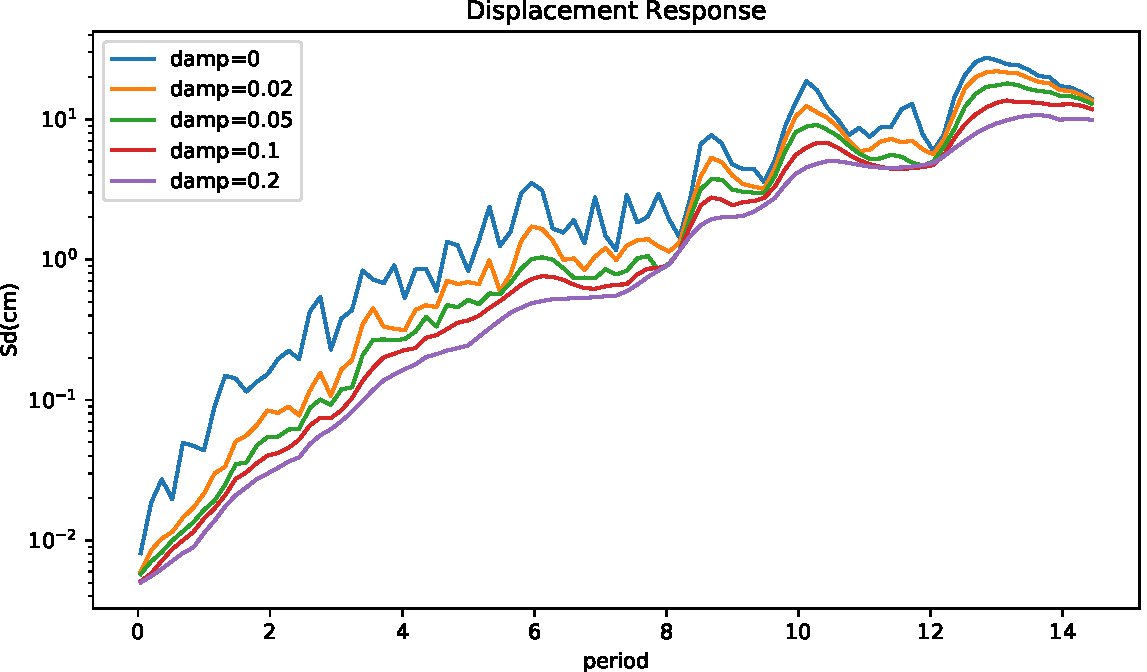
\includegraphics[width=4in, keepaspectratio]{figure/sd.pdf}
    \label{fig:sd}
\end{figure}

\end{homeworkProblem}


\end{document}
